\chapter{実装}\label{chap:implementation}

本章では、第\ref{chap:design}章で述べたプログラミング環境について述べる。
全体の概要について述べた後、個別の要素に関して述べる。

\section{Babascriptプログラミング環境}\label{babascriptux30d7ux30edux30b0ux30e9ux30dfux30f3ux30b0ux74b0ux5883}

Babascriptプログラミング環境は、人間とコンピュータへの指示を同じような記法で
実現・実行可能にするための仕組みである。 以下の要素によって実現する。

\begin{itemize}
\itemsep1pt\parskip0pt\parsep0pt
\item
  Babascript
\item
  Babascript Client
\item
  Node-Linda
\end{itemize}

Babascriptは人間への指示を記述可能にするプログラミングライブラリである。
Babascript Clientは、指示に対する実行結果を入力できるソフトウェアだ。
Node-Lindaは、Babascript及びBabascript
Clientの間のデータ通信の仲介サーバとして機能する。

以下のような手順で、処理が進む。

\begin{enumerate}
\def\labelenumi{\arabic{enumi}.}
\itemsep1pt\parskip0pt\parsep0pt
\item
  人への指示構文を実行する
\item
  指示内容がNode-Lindaサーバを経由してクライアントへと配信される
\item
  指示を受け取ったクライアントがユーザに処理を促す
\item
  指示実行者が、指示に従って行動し、その結果を入力する
\item
  Node-Lindaサーバを経由して実行元プログラムに入力された処理結果が送信される
\item
  プログラム側で指定されたコールバック関数が実行され、処理が継続される
\end{enumerate}

Babascriptプログラミング環境は、図\ref{fig:system_image}のように成り立つ。

\begin{figure}[htbp]
  \begin{center}
  \includegraphics[width=.8\linewidth,bb=0 0 563 151]{images/system_image.png}
  \end{center}
  \caption{システム全体像}
  \label{fig:system_image}
\end{figure}

以下の節において、個別の要素に関して詳しく述べる。

\section{Babascript}\label{babascript}

プログラムと人とのインタラクションを実現するためには、プログラム上で人間への指示を行える仕組みが必要だ。
そこで、Babascriptという、人間への指示構文を実装したオブジェクト(以下、人間オブジェクト)を宣言できるプログラミングライブラリを実装した。
BabascriptはJavascriptのサーバサイド実行環境であるNode.js及びプログラミング言語Ruby上で動作する。

\subsection{基本仕様}\label{ux57faux672cux4ed5ux69d8}

Babascriptでは、通常のメソッド実行とほぼ同じ記法で人間への指示を送ることができる。
例えば、図\ref{fig:babascript_sample}のようなプログラムによって、人間オブジェクトを宣言し、人間へ指示を送ることができる。

\begin{figure}[htbp]
  \begin{center}
  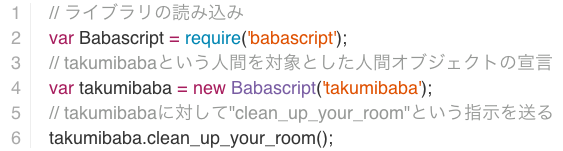
\includegraphics[width=.8\linewidth,bb=0 0 563 151]{images/babascript_sample.js.png}
  \end{center}
  \caption{人への命令構文}
  \label{fig:babascript_sample}
\end{figure}

人オブジェクトはインスタンス生成時にidを指定する必要がある。
人への命令構文は、このidを元に命令配信先を決定する。 例えば、id=baba
に命令を送りたければ、人オブジェクト宣言時の第一引数にはbabaという文字列を指定する。
指定したidに命令が配信されるため、Babascript
Client側でも同じidを指定する必要がある。
また、指定したidを監視しているクライアントが複数ある場合は、命令がラウンドロビン方式で配信される。
そのため、masuilabのような、特定のグループの人たちに命令を配信したいときなどにも利用可能である。

人間オブジェクトは、人間オブジェクトに定義されていないメソッドが実行されると、エラーを返さずに、人間への指示として解釈する。
そのため、実装されていないメソッド名であれば、あらゆる命令をメソッドとして表現し実行することが可能である。
例えば、「toString」や「call」等のメソッドは、javascriptにおいてはほぼすべてのオブジェクトが持つメソッドだ。
一方で、「clean\_up\_your\_room」や「bake\_bread」のようなメソッドは定義しない限りは存在しないメソッドである。
Babascriptは、この定義されていないメソッドをエラーとして評価せず、人への命令構文として評価する。

\begin{figure}[htbp]
  \begin{center}
  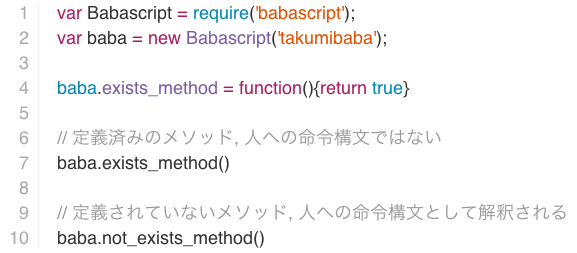
\includegraphics[width=.8\linewidth,bb=0 0 577 330]{images/methodmissing_sample.js.png}
  \end{center}
  \caption{人への命令構文}
  \label{fig:methodmissing_sample}
\end{figure}

また、図\ref{fig:babascript_exec_method}のように、execメソッドを使うことで指示を送ることも可能だ。
execメソッドを利用する場合は、第一引数に命令内容、第二引数にオプション情報、第三引数にコールバック関数を指定する。

\begin{figure}[htbp]
  \begin{center}
  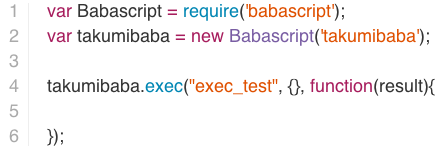
\includegraphics[width=.8\linewidth,bb=0 0 577 330]{images/babascript_exec_method.js.png}
  \end{center}
  \caption{人への命令構文}
  \label{fig:babascript_exec_method}
\end{figure}

オブジェクトに存在しないメソッドが呼び出された時に、特定のメソッドにその処理を委譲するような仕組みは、プログラミング言語Rubyにおいては
methodmissingと呼ばれる。
各言語によって名称は異なるが、類似する仕組みが存在する言語は複数存在する。

人間への指示として評価されたメソッドは、そのメソッド名と引数を元にしたタスク情報を生成し、タスク配信サーバへと送信する。
この際、メソッド名部分がユーザに命令として提示される文となる。
タスク情報は図\ref{fig:task_format}のように構成される。

\begin{figure}[htbp]
  \begin{center}
  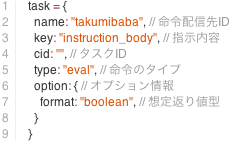
\includegraphics[width=.6\linewidth,bb=0 0 354 225]{images/task_format.js.png}
  \end{center}
  \caption{タスク情報}
  \label{fig:task_format}
\end{figure}

メソッド名が自由に設定できるため、内容は指示ではなく、質問のようなものもあり得るが、本研究では統一して指示と呼ぶ。
人への命令構文の第一引数にはオプション情報を指定する。
第二引数には人力処理の実行後に実行するコールバック関数を指定する。
このコールバック関数は、指示に対して何かしらの値が返されたときに実行される。

\subsection{オプション情報の付加}\label{ux30aaux30d7ux30b7ux30e7ux30f3ux60c5ux5831ux306eux4ed8ux52a0}

メソッド名以外に送信したい情報があるときには、第一引数にオプション情報としてオブジェクトを与える。
クライアントアプリケーション側でオプション情報を得ることができるため、このオプション情報に応じて
ユーザに提示する画面を変更するといったことが可能である。

オプション情報の例としては、返り値の型情報や、タイムアウト情報などが考えられる。
オプション情報は図\ref{fig:babascript_option}のように記述する。
図\ref{fig:babascript_option}の場合であれば、返り値の型はstringで、3分後までに返り値を得られなかった場合は、
人力処理を止め、第二引数で指定するコールバック関数を実行し、処理を続行させるといったことをオプション情報として記述している。

\begin{figure}[htbp]
  \begin{center}
  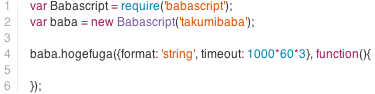
\includegraphics[width=.8\linewidth,bb=0 0 563 149]{images/babascript_option_sample.js.png}
  \end{center}
  \caption{オプション情報のサンプルソースコード}
  \label{fig:babascript_option}
\end{figure}

また、図\ref{fig:babascript_option_list}の場合であれば、listで指定した選択肢の中から選んで返り値を返す、といった指定が可能だ。

\begin{figure}[htbp]
  \begin{center}
  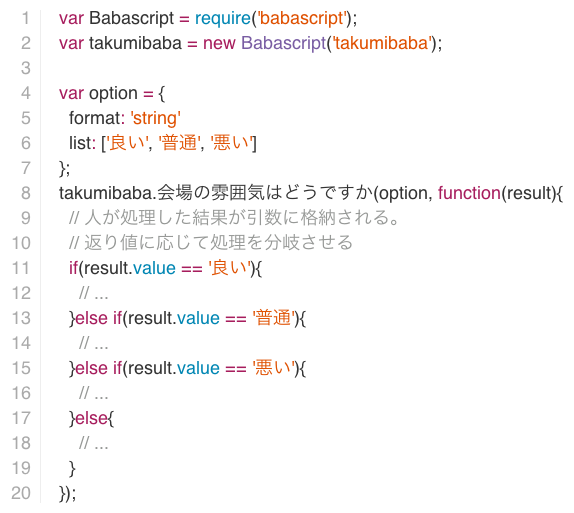
\includegraphics[width=.5\linewidth,bb=0 0 574 513]{images/babascript_option_list.js.png}
  \end{center}
  \caption{オプション情報のサンプルソースコード}
  \label{fig:babascript_option_list}
\end{figure}

オプション情報の中でもbroadcastというものは特別な情報として存在する。

オプション情報である第一引数は省略可能である。
省略した場合は、自動的に図\ref{fig:option_default}のようなオブジェクトが代入される。
図\ref{fig:option_default}のオプション情報の場合、返り値の型はBooleanで返すように指定できる。

\begin{figure}[htbp]
  \begin{center}
  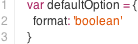
\includegraphics[width=.4\linewidth,bb=0 0 210 70]{images/option_default.js.png}
  \end{center}
  \caption{デフォルトのオプション情報}
  \label{fig:option_default}
\end{figure}

\subsection{コールバック関数の指定}\label{ux30b3ux30fcux30ebux30d0ux30c3ux30afux95a2ux6570ux306eux6307ux5b9a}

命令構文の第二引数にコールバック関数を指定すると、実行結果を取得した後にこのコールバック関数が呼ばれる
resultの中に処理結果が入ってる

\begin{figure}[htbp]
  \begin{center}
  \includegraphics[width=.5\linewidth,bb=0 0 574 513]{images/babascript_callback_func.js.png}
  \end{center}
  \caption{コールバック関数の指定}
  \label{fig:babascript_callback_func}
\end{figure}

人間は計算機の処理に比べて遅延しがちであるため、非同期を前提とした実装をしている

また、Promiseによる処理関数の指定も可能である。

\begin{figure}[htbp]
  \begin{center}
  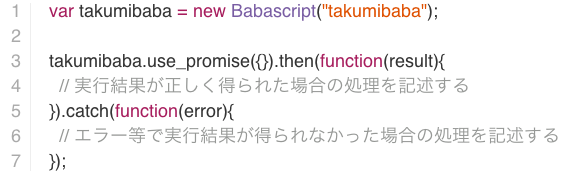
\includegraphics[width=.5\linewidth,bb=0 0 574 513]{images/babascript_promise.js.png}
  \end{center}
  \caption{コールバック関数の指定}
  \label{fig:babascript_promise}
\end{figure}

\subsection{コマンドラインでの利用}\label{ux30b3ux30deux30f3ux30c9ux30e9ux30a4ux30f3ux3067ux306eux5229ux7528}

Babascriptはコマンドラインツールとしても利用可能だ。
babaコマンドは、図\ref{fig:baba_command}のように利用することができる。
オプションeの直後に指示内容を、オプションnの直後に指示先のIDを指定する。
format情報などを付加したい場合は、オプションoの後に=の形で指定することができる。

\begin{figure}[htbp]
  \begin{center}
  
\includegraphics[width=.6\linewidth,bb=0 0 465 17]{images/baba_command.sh.png}
  \end{center}
  \caption{Babaコマンド}
  \label{fig:baba_command}
\end{figure}

図\ref{fig:baba_command_pipe}のように、pipeして使うなどの利用方法が考えられる。

\begin{figure}[htbp]
  \begin{center}
  \includegraphics[width=.4\linewidth,bb=0 0 465 17]{images/baba_command_pipe.sh.png}
  \end{center}
  \caption{Babaコマンドでpipeする}
  \label{fig:baba_command_pipe}
\end{figure}

\section{Babascript Client}\label{babascript-client}

Babascriptによって人への指示をプログラムに記述し、実行することが可能となったが、その指示を人に伝え、
処理結果を返させるためのアプリケーションが必要となる。
そこで、Babascript Clientというアプリケーション群を実装した。 Babascript
Clientは、Babascriptとの通信を担うサービス部と返り値の入力等を担うインターフェス部から構成される。
サービス部はJavascript上で動作する。
インタフェース部は、各種アプリケーションに応じて動作環境が異なるが、主にNode.js上とWebブラウザ上で動作する。

\subsection{サービス}\label{ux30b5ux30fcux30d3ux30b9}

サービス部は、主にBabascriptとのやりとり、つまり、命令の受け取りや返り値の送信などを担う。

命令を受け取ると、イベントを発行する

\begin{figure}[htbp]
  \begin{center}
  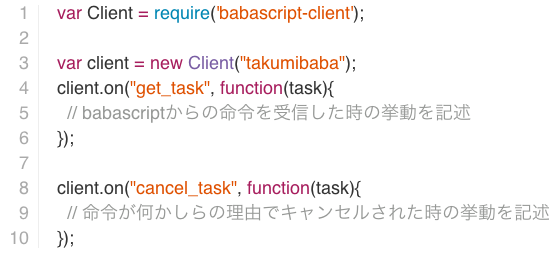
\includegraphics[width=.8\linewidth,bb=0 0 560 253]{images/babascript_client_service.js.png}
  \end{center}
  \caption{Babascript Client サービス部}
  \label{fig:babascript_client_service}
\end{figure}

何かしらの値を実行結果として返すときは、clientオブジェクトに実装されているretrnValueメソッドを用いる。
図\ref{fig:babascript_client_service_returnvalue}のように、第一引数に結果として返すものを指定する。

\begin{figure}[htbp]
  \begin{center}
  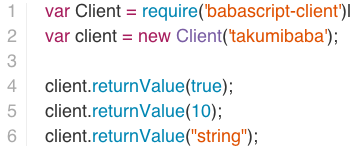
\includegraphics[width=.8\linewidth,bb=0 0 357 149]{images/babascript_client_service_returnvalue.js.png}
  \end{center}
  \caption{Babascript Client 処理結果を返すメソッド}
  \label{fig:babascript_client_service_returnvalue}
\end{figure}

実行結果情報として返すデータの例を図\ref{return_value_data}に示す。

\begin{figure}[htbp]
  \begin{center}
  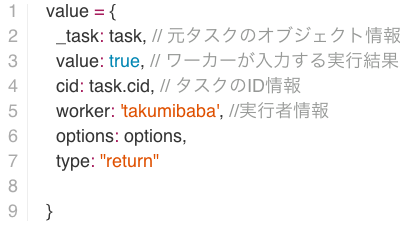
\includegraphics[width=.6\linewidth,bb=0 0 408 225]{images/return_value_data.js.png}
  \end{center}
  \caption{タスク情報}
  \label{fig:return_value_data}
\end{figure}

命令実行をキャンセルしたい場合は、cancelメソッドを用いる\ref{client_cancel_method}。
cancelメソッドの第一引数に、キャンセルする理由を指定することができる。

\begin{figure}[htbp]
  \begin{center}
  \includegraphics[width=.6\linewidth,bb=0 0 408 225]{images/client_cancel_method.js.png}
  \end{center}
  \caption{タスク情報}
  \label{fig:client_cancel_method}
\end{figure}

\subsection{ユーザインタフェース}\label{ux30e6ux30fcux30b6ux30a4ux30f3ux30bfux30d5ux30a7ux30fcux30b9}

ユーザとのインタラクションを行う。
命令をユーザに見せるのと、実際に実行結果を入力させる機能を持つ

サービス部と独立した実装のため、異なるデバイスや環境上でもインタフェース部を実装するだけでBabascript
Clientは構築可能である。
基本的には、指示内容と返り値の入力インタフェースをユーザに提示し、返り値の入力を受け付ける機能を担う。
この際、Babascriptの指示でオプション情報として返り値の型を指定していた場合、指定した型以外の入力を受け付けないような実装を行っている。
返り値の型は現在、Boolean, String, Numberに対応している。

例として、Webアプリケーション、コマンドライン・インタフェース、slackインタフェースを実装した。

\subsubsection{Webアプリケーション}\label{webux30a2ux30d7ux30eaux30b1ux30fcux30b7ux30e7ux30f3}

インタフェースの例として、Webアプリケーションとして実装した。
webブラウザ上で動作し、フレームワークにはBackbone.jsとMarionette.jsを利用した。
CSSはLESSを、HTMLはJadeで記述した。 Heroku上で稼働している。

システムは図\ref{fig:babascript_client_webapp_system}のように構成される。

\begin{figure}[htbp]
  \begin{center}
  \includegraphics[width=.3\linewidth,bb=0 0 273 402]{images/babascript_client_webapp_system.png}
  \end{center}
  \caption{Babascript Client webアプリケーションシステム図}
  \label{fig:babascript_client_webapp_system}
\end{figure}

Webインタフェースでは、指示内容に応じて提示インタフェースを変化させる実装をしている。
例えば、フォーマットにBooleanを指定していた場合、ユーザには trueボタンと
falseボタンが提示され、
どちらかのボタンを押すと、その結果が返り値としてプログラムに返される。
また、StringとNumberであれば、文字・数字の入力フォームと投稿ボタンが提示され、
投稿ボタンを押した際にフォームに入力されていた内容が返り値としてプログラムに返される。
実際に提示されるインタフェースの例を図\ref{fig:babascript_client_webapp_interface}に示す。

\begin{figure}[htbp]
  \begin{center}
  \includegraphics[width=.3\linewidth,bb=0 0 273 402]{images/babascript_client_webapp_interface.png}
  \end{center}
  \caption{Babascript Client Webアプリケーションインタフェース}
  \label{fig:babascript_client_webapp_interface}
\end{figure}

\subsubsection{チャットボット}\label{ux30c1ux30e3ux30c3ux30c8ux30dcux30c3ux30c8}

チャットサービス上で稼働するボットにBabascript Clientの機能を実装した。
ボットシステムにはHubotを採用した。
Hubotは様々なチャットサービスに対応しているが、Slackというチャットサービス上において運用している。
このボットシステムは、Heroku上で稼働している。
チャットボットのシステム図を図\ref{fig:babascript_client_hubot_system}に示す。

\begin{figure}[htbp]
  \begin{center}
  \includegraphics[width=.3\linewidth,bb=0 0 273 402]{images/babascript_client_hubot_system.png}
  \end{center}
  \caption{Hubotシステム図}
  \label{fig:babascript_client_hubot_system}
\end{figure}

チャットボットシステムは、ユーザからのメッセージによる問い合わせに応じて返答を行う。
返答の例を図\ref{fig:babascript_client_slack}に示す。

\begin{figure}[htbp]
  \begin{center}
  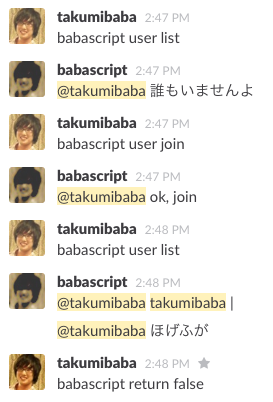
\includegraphics[width=.3\linewidth,bb=0 0 273 402]{images/babascript_client_slack.png}
  \end{center}
  \caption{Babascript Client Slackインタフェース}
  \label{fig:babascript_client_slack}
\end{figure}

チャットボットシステムの問い合わせに対する動作のリストを表\ref{tb:babscript_hubot_mention}に示す。

チャットボットインタフェースでは、Webアプリケーションの場合と違い、
提示するインタフェースを返り値の型に応じて変化させるといったことができない。
そのため、ユーザにとっては値を返しにくくなっているが、普段利用しているチャットサービス上で
Babascript
Clientの機能を利用できるということは有用なことであると考える。

\section{通信手法}\label{ux901aux4fe1ux624bux6cd5}

BabascriptとBabascript
Client間の通信のために、仲介サーバとしてNode-Lindaを利用する。
通信手法はデバイスごとに利用可能な手法が異なったり限定されるため、プラガブルにする必要がある。
そこで、シンプルで接続方式の追加が簡単に可能な実装となっているNode-Lindaを仲介サーバソフトウェアとして採用した。

Babascript及びBabascript
ClientがNode-Lindaに接続するために実装されたモジュールを、Babascript
Adapterと呼ぶ。
このAdapterは簡単に切り替えが可能で、かつ他の実装に影響を与えることがないように設計されている。
Babascript及びBabascript
ClientはこのAdapterを介してNode-Lindaに接続し、情報のやりとりを行う。

本節では、この仲介サーバとして用いるNode-Lindaについて述べた後、2種類のBabascript
Adapterを紹介する。

\subsection{Node-Linda}\label{node-linda}

Node-Linda\cite{node-linda}は、分散並列処理のための仕組みであるLinda\cite{linda}をNode.js上に実装したものだ。
Lindaは、タプルスペースという共有メモリを用いてプロセス間でデータの通信を行う並列処理のためのモデルだ。
Node-Lindaでは、Lindaを拡張し、ネットワーク経由でも利用できるようにしている。
ネットワーク経由での利用のため、あらゆるプログラミング言語から利用可能だ。
接続のためのプログラムさえ記述すれば、あらゆるデバイスがNode-Lindaに接続可能である。
Linda及びNode-Lindaのタプル空間への操作を表\ref{table:tuple-management}にまとめる。

\begin{longtable}[c]{@{}lcc@{}}
\caption{Linda及びNode-Lindaのタプル空間への操作
\label{table:tuple-managemnet}}\tabularnewline
\toprule
操作 & Linda & Node-Linda\tabularnewline
\midrule
\endfirsthead
\toprule
操作 & Linda & Node-Linda\tabularnewline
\midrule
\endhead
書き込み & out & write\tabularnewline
読み込み & rd & read\tabularnewline
読み込みつつ削除 & in & take\tabularnewline
ブロックして読み込み & rdp & -\tabularnewline
ブロックして読み込みつつ削除 & inp & -\tabularnewline
書き込みを読み続ける & - & watch\tabularnewline
\bottomrule
\end{longtable}

watch操作は従来のLindaの仕様にはなく、Node-Linda独自の仕様である。
また、Node-Lindaでは非同期処理が前提となっており、ブロック処理は仕様から削除されている。

実世界コンピューティングでの利用を前提としており、様々なセンサーやアクチュエータが接続することが想定される。
Babascriptによる人間の指示実行結果も、センサーやアクチュエータの処理を同じようにNode-Linda上で共有される。
つまり、Node-Linda上において人間はセンサーやアクチュエータと同じような存在になる。

Node-Lindaの各操作は、図\ref{fig:linda-usage}のようなプログラムで実現する。

\begin{figure}[htbp]
  \begin{center}
    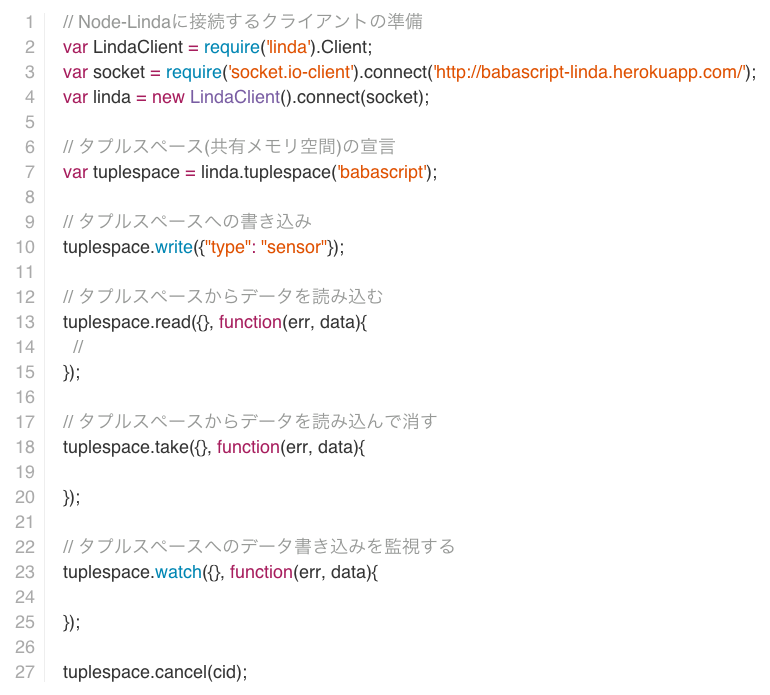
\includegraphics[width=.7\linewidth,bb=0 0 770 695]{images/linda-usage.js.png}
  \end{center}
  \caption{Node-Lindaへの接続方法}
  \label{fig:linda-usage}
\end{figure}

\subsection{Socket.IO Adapter}\label{socket.io-adapter}

Socket.IO
Adapterは、リアルタイム通信のためのライブラリであるSocket.IO\footnote{http://socket.io/}を用いて
Node-Lindaに接続するためのAdapterだ。
WebsocketもしくはXHR-Pollingによって常にNode-Lindaサーバと通信をし続ける。
全ての処理はSocket.IOによる通信によって実現する。

常時通信している都合上、バッテリー消費の問題が生じたり、デバイスによっては通信を強制的に切断されてしまうことがある。
Socket.IO Adapterは、接続環境が良好な状態での利用が望ましい。
例えば、常設型のコンピュータ等においての利用が想定される。

構成図を図\ref{fig:socket.io-adapter}に示す。

\subsection{PushNotification Adapter}\label{pushnotification-adapter}

PushNotification Adapter は、HTTP
RequestとPushNotificationを用いてNode-Lindaと通信を行うためのAdapterだ。
Node-Lindaへのタプル操作はHTTP Requestの実行によって実現する。
Node-Linda側からAdapter側への通信には、PushNotificationを用いる。 Amazon
AWS
SimpleNotificationService\footnote{http://aws.amazon.com/jp/sns/}を利用し、
PushNotificationを実現している。 PushNotification
Adapterを利用するためには、Node-Linda側でPushNotification
Adapter用のライブラリを読み込む必要がある。

PushNotification
Adapterは、モバイルデバイス等の常時接続が難しいデバイス上で、可能な限りリアルタイムなやりとりを実現するために
実装された通信モジュールだ。
主にAndroidやiPhone等のモバイルデバイスからNode-Lindaと接続する際に利用する。

構成図を図\ref{fig:pushnotification-adapter}に示す。

\section{まとめ}\label{ux307eux3068ux3081}

人間と計算機の処理を融合させたプログラミング環境の具体的な実装や利用方法について述べた。
